\documentclass[a4 122pt]{article}

\usepackage{color}
\usepackage{polski}
\usepackage[utf8]{inputenc}
\usepackage{amsmath}
\usepackage{amsthm}
\usepackage{todonotes}
\usepackage{geometry}
\usepackage{hyperref}
\geometry{
  body={6.5in, 8.5in},
  left=0.7in,
  top=0.8in,
  bottom=0.8in
}
\usepackage[pdftex]{graphicx}
\usepackage{sidecap}
\usepackage[linesnumbered, vlined]{algorithm2e}
\newtheorem{twierdzenie}{Twierdzenie}
\newtheorem{definicja}{Definicja}
% zmiana caption dla algorytmu
\usepackage{caption}% http://ctan.org/pkg/caption
\newenvironment{algorytm}[1][htb]
  {\renewcommand{\algorithmcfname}{Algorytm}%
   \begin{algorithm}[#1]%
  }{\end{algorithm}}


\title{Planarność grafu}
\author{Paweł Sokołowski\\Michał Kaszlej}


\begin{document}


\maketitle

	\section{Cel projektu}

		Celem projektu jest napisanie algorytmu heurystycznego sprawdzającego czy zadany graf jest planarny.
		Według twierdzenia podanego w książce (Wilson, 1998):

		\begin{figure}[h]
			\begin{center}
				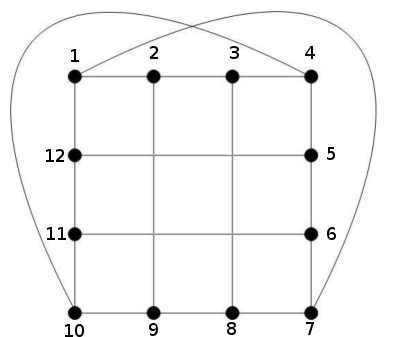
\includegraphics[width=0.5\textwidth]{include/graf.png}
				\caption{Zadany graf}
			\end{center}
		\end{figure}


		Dany graf jest planarny wtedy i tylko wtedy, gdy nie zawiera podgrafu ściągalnego do grafu $K_{3.3}$ lub do grafu $ K_5 $

	\section{Język programowania} 

		Algorytm zostanie zaimplementowany za pomocą języka C\#.

	\section{Algorytm}

		Algorytm rozwiązujący zadany problem zostanie wybrany w dalszej fazie projektu.

	\pagebreak

	\section{Opis algorytmu}	
	Algorytmem, który zostanie zaimplementowany w celu sprawdzenia czy zadany graf jest planarny jest test planarności przy użyciu twierdzena Wagnera: 
	\begin{twierdzenie}
	Dany graf jest planarny wtedy i tylko wtedy, gdy nie zawiera podgrafu ściągalnego do grafu $K_{3.3}$ lub do grafu $ K_5 $
	\end{twierdzenie}
	Implementacja algorytmu wywodzi się wprost z powyższego twierdzenia. 
	Polegała będzie ona na dokonywaniu operacji ściągania grafu do podgrafu o 5 lub 6 wierzchołkach.
	Jeżeli uda się w ten sposób utworzyć graf $ K_5 $ lub $K_{3.3}$ oznaczało to będzie, że wejściowy graf nie jest planarny.
	Poniżej znajduje się pseudokod algorytmu.
	
	\begin{algorytm}[H]
	\newcommand{\forcond}{$i=0$ \KwTo $n$}
	\SetKwFunction{Fn}{JestPlanarny}
	\Fn{graf g}\Begin{
	
		\KwData{Testowany graf}
		\KwResult{Czy testowany graf jest planarny}
		\If{g posiada 6 wierzchołków}{
			Sprawdź czy graf jest $K_{3.3}$\;
		}
		\If{g posiada 5 wierzchołków}{
			Sprawdź czy jest $K_5$\;
		}
		\If{graf posiada więcej niż 5 wierzchołków}{
			\ForEach{krawędź e grafu g}{
				h $\leftarrow$ zbuduj graf poprzez ściągnięcie krawędzi e z grafu g\;
				\Fn{h}\;
			}
		}
	}
	\caption{Pseudokod algorytmu}
	\end{algorytm}
	
	Linie 1-6 algorytmu wydają się dosyć oczywiste. 
	Jeżeli mamy doczynienia z grafem pięcio lub sześcio wierzchołkowym sprawdzane jest odpowiednio czy nie jest to odpowiednio $K_5$ lub $K_{3.3}$. 
	W linii 8 następuje iteracja po wszystkich krawędziach grafu. 
	Najistotniejszym fragmentem algorytmu wydaje się być linia 9. 
	Budowany jest tam nowy graf poprzez "ściągnięcie" danej krawędzi. 
	Sama operacja zostanie opisana w dalszej części pracy.
	
	\subsection{Operacja ściągnięcia}
		Ściąganie wzdłuż krawędzi polega na utożsamianiu wierzchołków, które łączy dana krawędź i pomijaniu ewentualnych pętli. 
 		
		\begin{definicja}
			Mówimy, że graf $G_1$ jest ściągalny do $G_2$, jeśli $G_2$ można otrzymać z $G_1$ poprzez skończony ciąg operacji ściągania wzdłuż krawędzi.
		\end{definicja}
		
		Z \textbf{Twierdzenia 1} wiemy, że jeżeli uda nam się ściągnąć graf wejściowy do $K_5$ lub $K_{3,3}$ to nie jest planarny. 
	
	\subsection{Struktury danych}

		Graf reprezentowany będzie za pomocą listy sąsiedztwa. 
		W reprezentacji tej, struktura przedstawiająca wierzchołek będzie składała się z jego identyfikatora oraz listy jego sąsiadów. 
		Sam graf będzie zbudowany z listy wierzchołków. 
		Reprezentacja ta pozwoli na budowanie grafu poprzez ściągnięcie krawędzi w czasie $O(m)$.
	
	\subsection{Historia operacji}
		Celem zadania jest próba znalezienia podgrafu ściągalnego do $K_5$ lub $K_{3,3}$, aby odpowiedzieć na pytanie czy dany graf jest planarny. 
		Nie wystarczy więc aby projektowany algorytm zwracał jedynie binarną odpowiedź, tak lub nie, musi w przypadku stwierdzenia nieplanarności zwrócić podgraf ściągalny do $K_5$ lub $K_{3,3}$.
		Aby mieć możliwość odtworzenia takiego podgrafu (w trakcie działania algorytmu zmieniana jest struktura grafu, usuwane są krawędzie i wierzchołki) podczas każdego zejścia rekurencyjnego zapamiętywana będzie historia ściągniętych krawędzi. 
		Umożliwi to odtworzenie szukanego podgrafu w zadanym grafie.
	
	\subsection{Złożoność}
	
		Istnieje, szereg algorytmów pozwalących na sprawdzenie planarności grafu.
		Od roku 1974 istnieją algorytmy o złożoności liniowej $O(n)$ w tym np. metody Hopcroft, Tarjan czy Boye, Myrvold.
		Są to metody bardzo skomplikowane, wymagające żmudnej, czasochłonnej implementacji.
		
		Prostszy w implementacji jest algorytm korzystający z obserwacji dotyczących cyklów i segmentów w grafach planarnych. 
		Jest on mniej wydajny niż wspominane powyżej algorytmy, ale jego złożoność jest również wielomianowa - rzędu $O(n^3)$. 
		Niestety, algorytm ten nie mógł być zastosowany, ponieważ w przypadku stwierdzenia nieplanarności nie zwraca on podgrafu ściągalnego do $K_5$ lub $K_{3, 3}$.
		
		Jako, że zadanie projektowe zdefiniowane zostało dla grafu o 12 wierzchołkach - zdecydowaliśmy, że zastosowanie tak skomplikowanych algorytmów nie jest tu zasadne. 
		Zaprezentowane w ninejszej pracy rozwiązanie osiąga wydajność na poziomie $O(m!)$.

	\pagebreak
	
\section{Realizacja projektu}

		
	\subsection{Implementacja}

		Algorytm zaimplementowany został w technologii .NET Framework. Użytym językiem programowanie był C\#.
		Kod źródłowy dostępny jest za pośrednictwem portalu github: \url{https://github.com/sokolowskip/WMH}.
		Prace nad implementacją przeprowadzono przy użyciu rosproszonego systemu kontroli wersji git.

	\subsection{Sposób uruchomienia}
	
		Aplikacja relizująca opisany algorytm i sprawdzająca czy zadany graf jest planarny została nazwana \texttt{PlanarityTesting}. 
		Jedynym parametrem wejściowym programu jest nazwa pliku zawierającego tekstowy opis grafu. Program uruchamiany jest za pomocą polecenia:
		\begin{verbatim}
		PlanarityTesting fileName
		\end{verbatim}
	\subsection{Format danych wejściowych} \label{sec:format}
	
		Zadany graf w przyjętej reprezentacji wygląda następująco:
		\begin{SCfigure}[\sidecaptionrelwidth][h!]
			\centering
			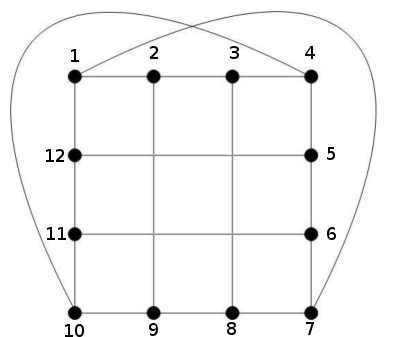
\includegraphics[width=0.3\textwidth]{include/graf.png}
			\caption*
{
\texttt{1: 2,7,12\\
2: 1,3,9\\
3: 2,4,8\\
4: 3,5,10\\
5: 4,6,12\\
6: 5,7,11\\
7: 1,6,8\\
8: 4,7,9\\
9: 2,8,10\\
10: 4,9,11\\
11: 6,10,12\\
12: 1,5,11}}
		\end{SCfigure}
	\subsection{Wyjście programu}

	\subsection{Reprezentacja grafu}

\subsection{Testy}

	\subsection{Sposoby testowania}

		Podstawowym zadaniem stojącym przed projektem było stwierdzenie czy zadany graf jest planarny.
		W celu weryfikacji, czy implementacja działa także dla innych algorytmów - przygotowano dane testowe.
		
		Dla grafów testowych znane jest prawidłowe wyjście programu. Weryfikacja działania programu polegała na wprowadzaniu kolejno danych testowych i weryfikacji wyjścia programu.		

	\subsection{Grafy użyte do testów}

\begin{verbatim}
graph1.txt
1: 2, 3
2: 1, 3
3: 1, 2
Graf planarny
\end{verbatim}

\begin{verbatim}
graph2.txt
1: 5,6,7
2: 4,5,6
3: 4,5,12
4: 2,3,7
5: 1,2,3
6: 1,2,10,8
7: 1,4,8,9
8: 7,9,6
9: 7,8
10: 11,6
11: 10,12
12: 3, 11
Graf nie jest planarny
\end{verbatim}
	\subsection{Wyniki testów}

\section{Wnioski}

	\subsection{Efektywność algorytmu największym wyzwaniem}
	\subsection{Wykorzystanie kryteriów eulera}

\section{Bibliografia}

		Wilson R. J., Wprowadzenie do teorii grafów, Warszawa 1998, Wydawnictwo Naukowe PWN.\\[0.3cm]
		\url{www.win.tue.nl/~nikhil/courses/2012/2WO08/lecture5.pdf}, ost. wiz. 17.12.2013.\\[0.3cm]
		\url{http://www.geeksforgeeks.org/bipartite-graph/}, ost. wiz. 20.12.2013.

\end{document}	
